

\section{Surface visualization techniques}

In this section we will focus on different surface visualization techniques. Roughly we can divide surface mesh generation into \emph{model-based} and \emph{model-free}.

The model-based mesh generation makes some assumptions about the model, in our case about the vascular system.
In paculiar it makes assumptions about the topological structure, the observed junctions and the profiles of vessels. The topological structure is mostly represented by a graph and limited to a tree like representation. Also the observed junctions often are limited to certain kinds of junctions like bifurcations. Finally the profiles of the vessels are simplified to circular or eliptical structures.
All this simplifications and assumptions can help to speed up the process of surface generation, to make it more reliable or more visually pleasing or even transform the underlying data into more usable data for further processing. The downside is that model-based meshes do not resemble the underlying data as accurate as it could be done and also sometimes simplify the underlying data too much such that essential features are lost.
Especially when diagnoses of vascular degenerations or similar detail based inspections need to be done model-based approaches may not provide enough vivid information of the underlying data.

Here model-free mesh generation comes into play. The goal here is to retain as much of the underlying data as possible. But without a underlying model the extraction and creation of the mesh is more time consuming and cumbersome. Moreover unwanted results can arise if the underlying data suffers from noise or other failures in capturing. So care must be taken at the decision what for data is extracted and finally represented in the resulting mesh.

From the literature observed we determined that most of the methods require at some points a skeletonization of the underlying data. For now we assume that the underlying data consists of a voxel model that represents a density field of captured values. As model-based methods require a model, all of the observed methods require an extraction of a skeleton prior to the actual mesh generation. In regards of skeletonization the interested reader is reffered to Ebert et al.~\cite{ebert2002augmented} or  Strzodka et al.~\cite{strzodka2004generalized}.

As seen model-based mesh generation is based more or less on geometrical assumptions and reasoning on the model.
Volkau et al.~\cite{volkau2005geometric} for instance models a cerebral arterial model from segmented and skeletonized angiographic data. He constructs a vascular structure consisting of tube segments and bifurcations, so this model-based approach limits the domain of representable data quite hard in regards of branching possibilites. The centerline is smoothed with a sliding average filter to prevent problems with outliers and the two kinds of topologies, namely tubular and B-Subdivison based ones, are combined to form the complete vessel structure.

A connected graph is established that captures also the blood flow direction. This is done by splitting it up into two connected tree structures where one is designated as inflow structure. The model shapes the tube segments with decreasing radius with respect to the bloodflow as well as it captures radii change at bifurcations. This is based on statistical data. Radii at bifurcations are approximated with an exponential function whrereas radii evolution at tubular parts are done via linear regression. At connection points C1 continuity is established via further constraints. So no abnormal cross section shape or diameter will show up easily in the final result.

\begin{figure}[h]
	\centering
	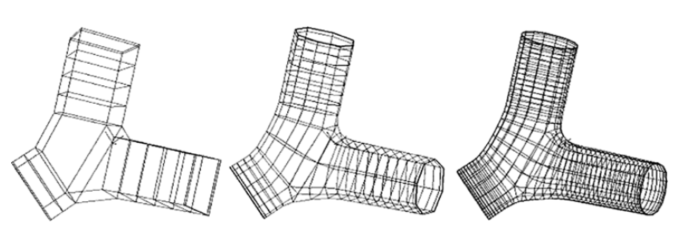
\includegraphics[width=0.8\textwidth]{./Images/B-subdivision_refinement.png} \\
	\caption{Example of refinement with B-subdivision.}
	\cite{volkau2005geometric}
	\label{fig:B-subdivision_refinement}
\end{figure}

The bifurcations themselves are constructed based on B-subdivison. The generation of quadrangles of a bifurcation till the overlapping internal part is shown in figure \ref{fig:B-subdivision_refinement}. Internal parts are subdivided to fit the outer subdivison. Problems with this scheme arise when all three vessels at the bifurcation form a close to orthogonal connection, where the inner face will be undefined. Also the B-subdivision of tubular segments show problems, namely self intersections when the radius of of curvature is smaller than the radius of the tube, shown in figure \ref{fig:Fold_of_vessel}.
Further problems mentioned are 'oversampling' or unrealistic sampling of bifurcations according to a too croase sample pattern or problems with centerline smoothing in very jaggy areas as an acceptable smoothing also will remove esential features of the unterlying vascular structure.  

\begin{figure}[h]
	\centering
	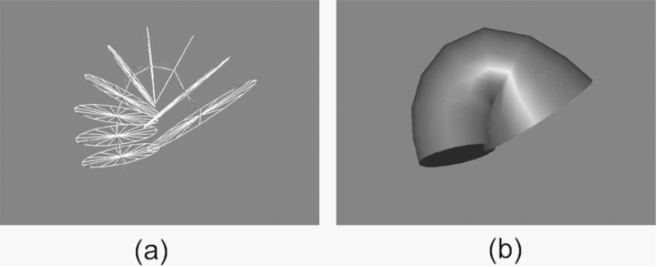
\includegraphics[width=0.8\textwidth]{./Images/Fold_of_vessel.png} \\
	\caption{Fold of vessel when curvature is higher than tube radius.}
	\cite{volkau2005geometric}
	\label{fig:Fold_of_vessel}
\end{figure}

\begin{figure}[h]
	\centering
	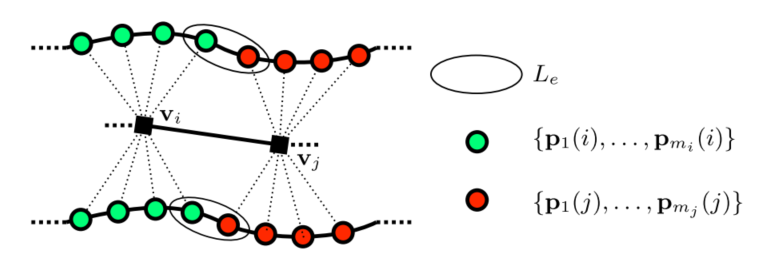
\includegraphics[width=0.8\textwidth]{./Images/Estimate_thickness.png} \\
	\caption{Estimation of thickness of graph edges.}
	\cite{sibbing2012topology}
	\label{fig:Estimate_thickness}
\end{figure}

Another geometry based modelling approach is provided by Sibbing et al.~\cite{sibbing2012topology}.
His work is focusing on quad meshes as they are visually more pleasant, require fewer elements and can produce more stable results in further processing, like FEM. Here the topologically correct extraction of the branching structure is done from a post-processed triangle mesh that is generated from an adapted \emph{Marching Cubes} algorithm based on the interior voxels which are identified via a variant of the \emph{Level Set} method. The extracted mesh is shrinked to a close to one dimensional structure that serves as basis for a tree based graph as well as for radius estimation along its edges, see figure \ref{fig:Estimate_thickness}. Further the graph is used to subdivide the triangle mesh into tubular parts and parts with one or more furcations with appropriate placed cutting planes. The so called \emph{interfaces} are 2D polygons between adjacent segments. They are defined by the intersection of cutting planes with the triangular mesh. 

Quad meshes for the junctions are created with the \emph{Mixed Integer Quadrangulation} by Bommes et al.~\cite{bommes2009mixed}. The quads are just required to align with the defined boundary to generate radially arranged quads.

\begin{figure}[h]
	\centering
	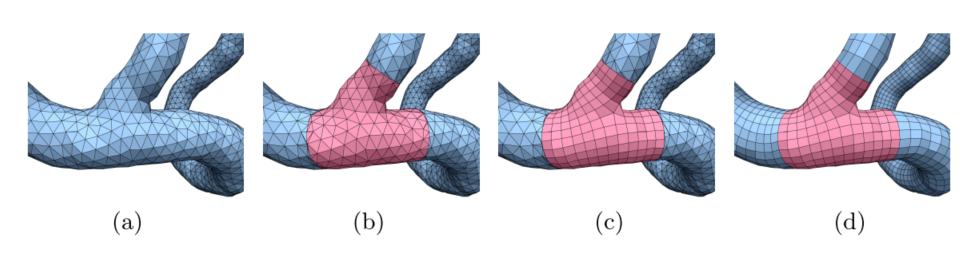
\includegraphics[width=0.8\textwidth]{./Images/Remeshing_stage.png} \\
	\caption{ (a) The input to our remeshing stage is a smoothed and resampled version of the mesh extracted using the Marching Cubes Algorithm. (b) The mesh is partitioned into junction and tube components. The cuts insert additional vertices at the respective interfaces. (c) We remesh the junctions yielding a fair quad layout. (d) Tubes are remeshed, such that the final mesh is a quad dominant mesh.}
	\cite{sibbing2012topology}
	\label{fig:Remeshing_stage}
\end{figure}

Tubes now only have to provide a smooth transition between two interfaces with a possibly different number of vertices. The rings of the tubes are generated out of equidistant iso-contours on the harmonic scalar field on the tube. Triangles are introduced between so called transition rings to compensate for the difference in vertices. The distribution of the transition rings as well as the distribution of the triangles around the tube in a transition case is done via adaption of the Bresenham line rasterizaion algorithm. Stretching of quads along the tube axis as well as rotations of the rings to get configurations with almost $90$ degree angles in the quads, yields close to optimal quad dominant meshes. The advantage of this reconstruction is the smoothing of unwanted artifacts on the original triangle mesh as well as the already shown properties of quad meshes, see figure \ref{fig:Remeshing_stage}.

%Describe skeletonization, e.g Topology aware Quad Dominant Meshing p.4f